% ex: tw=74 ts=2 sw=2 noet sts=2
\documentclass[10pt]{article}
\usepackage[utf8]{inputenc}
\usepackage{amsmath}
\usepackage{xkeyval}
\usepackage[bookmarksnumbered,frenchlinks]{hyperref}
%\hypersetup{pdfborder=0 0 0}
\usepackage{multirow}
\usepackage[english]{babel}
\usepackage{fullpage}
\usepackage{tabulary}
\usepackage{tabularx}
%\usepackage{natbib}
\usepackage[all]{hypcap}
\usepackage{hyperref}
\usepackage{framed}
\usepackage{fullpage}
\usepackage{graphicx}
\usepackage{listings}
\usepackage{subfig}
\usepackage{verbatim}
\usepackage{float}
%\floatstyle{boxed} 
%\restylefloat{figure}
\title{\textbf{Experiment 1} \\
	Activity 2}
\author{Cody Schafer}
\date{\today}
\begin{document}
\maketitle
\section{Introduction}
% An Introduction containing a brief description of the lab

	This lab will familiarize you with the voltage transfer
	characteristics and switching times of a BJT inverter.  There are
	two different activities.  In the first activity you will look at
	the operation of a diode and the capacitances at the p-n junction.
	In the second, the operation of a BJT inverter circuit, and
	different ways to eliminate delays in input response will be
	explored.    

\section{Activities}
% A description of each activity and what was accomplished

	In the second activity (activity 1 was completed in lab 1),
	inverters were constructed using a BJT an a resistor. Various
	properties of this circuit were noted, and then, to decrease the
	storage times, the addition of a diode and then the addition of a
	capacitor to the circuit was tested.

\section{Data}
% Any data, tables, or graphs developed in the course of the lab

	\subsection{Determination of Saturation Voltage}
	\textbf{See Anthony's report for this section.}

	\begin{comment}
	5V was attached to $V_{cc}$ and $V_i$ was varied from 0 upward by
	increments of 0.2V until the transistor turned on.

	\begin{table}[H]
		\centering
		\subfloat[TIP31 transistor data]{
			\begin{tabular}{c|c|c}
				$V_i$ & $V_{BE}$ & $V_o$ / $V_{CE}$ \\ \hline
				0.0	& 0.010 & 5.060 \\
				0.2	& 0.212	& 5.061 \\
				0.4 & 0.414 & 5.061 \\
				0.6 & 0.58	& 4.375 \\
				0.8	& 0.627 & 0.813 \\
				1.0	& 0.634	& 0.087 \\
				1.2 & 0.636 & 0.067 \\
				1.4 & 0.639 & 0.056 \\
				1.6 & 0.641 & 0.048 \\
				1.8 & 0.644 & 0.043
			\end{tabular}
		}
		\qquad
		\subfloat[2N3904 transistor data]{
			\begin{tabular}{c|c|c}
				$V_i$ & $V_{BE}$ & $V_o$ / $V_{CE}$ \\ \hline
				0.0	& 0.012 & 5.067 \\
				0.2	& 0.213	& 5.067 \\
				0.4 & 0.414 & 5.067 \\
				0.6 & 0.614	& 5.041 \\
				0.8	& 0.706 & 2.123 \\
				1.0	& 0.760	& 0.170 \\
				1.2 & 0.762 & 0.140 \\
				1.4 & 0.763 & 0.126 \\
				1.6 & 0.765 & 0.117 \\
				1.8 & 0.766 & 0.111 \\
				2.0 & 0.767 & 0.106 \\
				2.2 & 0.769 & 0.101 \\
				2.4 & 0.770 & 0.098 \\
				2.6 & 0.770 & 0.095 \\
				2.8 & 0.771 & 0.092 \\
				3.0 & 0.772 & 0.090
			\end{tabular}
		}

		\caption{Data recorded from raising the $V_i$ in 0.2V increments.}
		\label{tbl:1}
	\end{table}
	\end{comment}

	\subsection{Second Part}
	\textbf{See Anthony's report for this section.}

	\subsection{Third Part}
		\begin{table}[H]
			\centering
			\begin{tabular}{*{6}{c|}c}
			Transistor & $V_{OH}$ & $V_{OL}$ & $t_{d1}$ & $t_f$ & $t_s$ & $t_r$
			\\ \hline

			TIP31 & 5.08 & 0.320 & 197ns & 549ns & 0 & 3.49us \\

			2N3904 & 5 & 0.440 & 58.7ns & 421ns & 0 & 2.57us \\

			\end{tabular}
			\caption{Timing values obtained with 10KHz input square wave}
		\end{table}

		\begin{table}[H]
			\centering
			\begin{tabular}{*{4}{c|}c}
				Transistor & $I_{RB}$ & $I_{BE} + I_{CB}$ & $I_{BE}$ & $I_{CB}$ \\ \hline
				TIP31  & 2.214mA & 2.2233 & 0.1193mA & 2.104mA \\
				2N3904 & 2.152mA & 2.2403mA & 0.2425mA & 1.9978mA \\
			\end{tabular}
			\caption{Currents obtained when input $V_i$ is 5V (DC)}
			\label{tbl:3}
		\end{table}

		\begin{figure}[H]
			\centering
			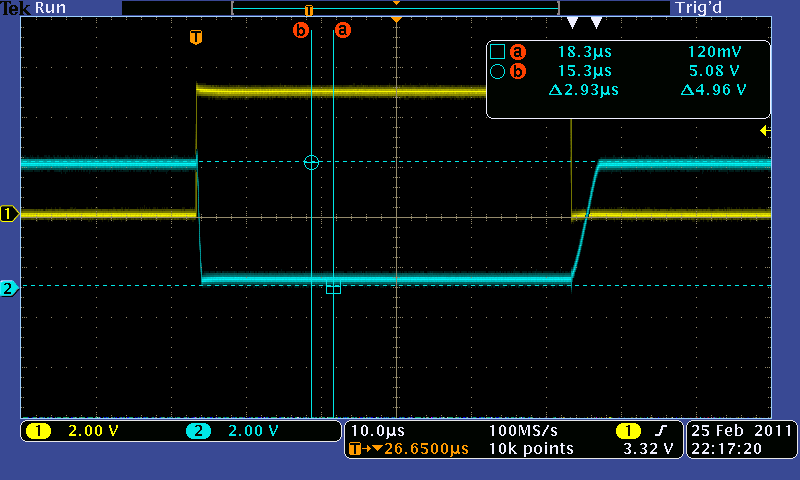
\includegraphics[width=4.5in]{wave_3_tip31.png}
			\caption{TIP31 Wave with diode inserted}
			\label{fig:tip31-3}
		\end{figure}

		\begin{figure}[H]
			\centering
			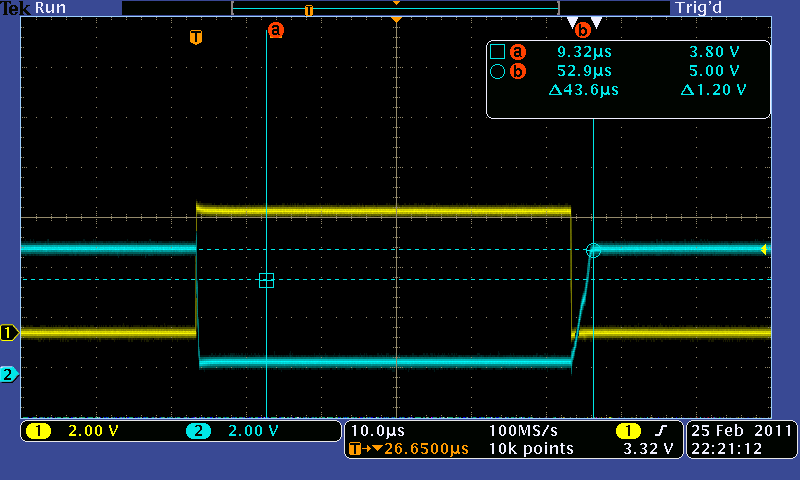
\includegraphics[width=4.5in]{wave_3_3904.png}
			\caption{2N3904 Wave with diode inserted}
			\label{fig:2N-3}
		\end{figure}

	\subsection{Fourth Part}
		\begin{table}[H]
			\centering
			\begin{tabular}{*{4}{c|}c}
				Transistor & $T_d$ & $T_f$ & $T_s$ & $T_r$ \\ \hline

				TIP31 & 53.3ns & 20.0ns & 2.63us & 181ns \\
				2N3904 & 29.3ns & 17.3ns & 0 & 151ns \\
			\end{tabular}
			\caption{Timing data with capacitor added.}
			\label{tbl:4}
		\end{table}
		
		\begin{figure}[H]
			\subfloat{
				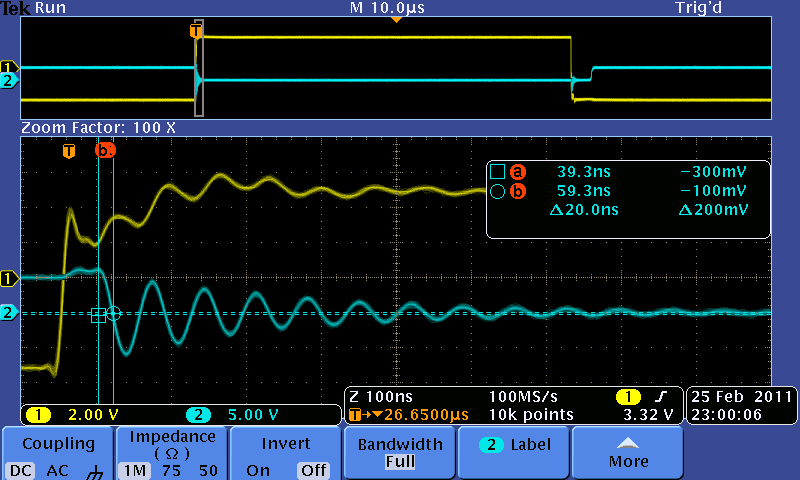
\includegraphics[width=3.2in]{wave_4_tip31_a.png}
			}
			\subfloat{
				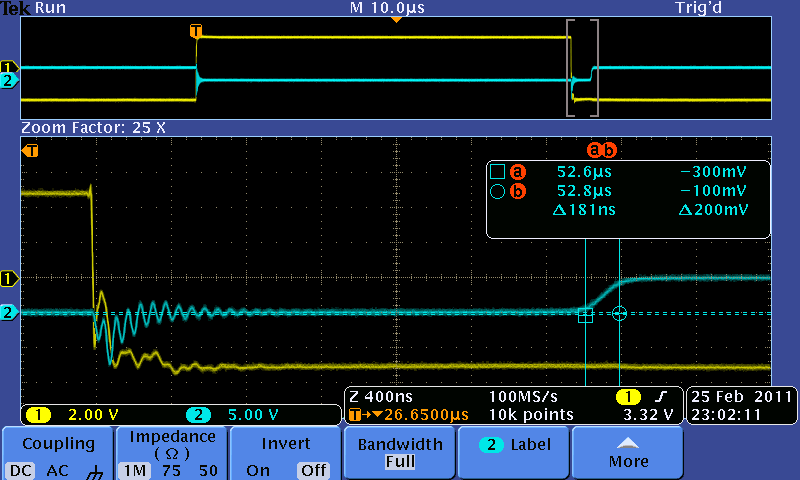
\includegraphics[width=3.2in]{wave_4_tip31_b.png}
			}
			\caption{TIP31 Wave with capacitor inserted}
			\label{fig:tip31-4}
		\end{figure}

		\begin{figure}[H]
			\subfloat{
				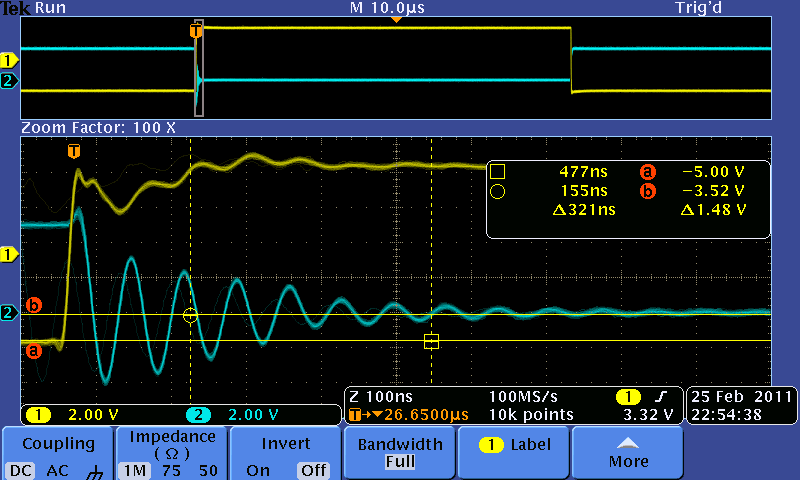
\includegraphics[width=3.2in]{wave_4_3904_a.png}
			}
			\subfloat{
				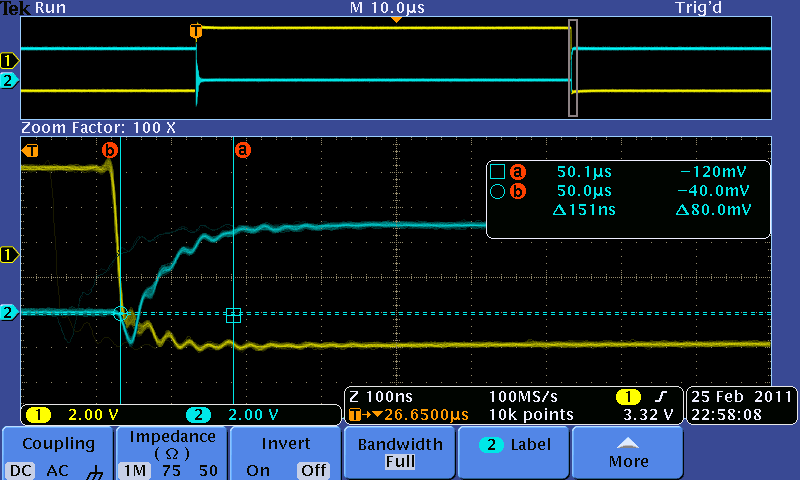
\includegraphics[width=3.2in]{wave_4_3904_b.png}
			}
			\caption{2N3904 Wave with capacitor inserted}
			\label{fig:2N-4}
		\end{figure}

\section{Discussion}

\subsection{DC analysis of the Inverter}

From the tables of recorded values, we can see that the cut in voltage for
each of the tested transistors occurs around the same voltage values.
Cut-in is the voltage at which the transistor transitions from cut-off to
active mode, meaning current begins flowing from the collector to the
emitter. The TIP31 showed a cut-in voltage of 1.0V and the 2N3904 showed
an identical cut-in of 1.0V. These voltages are the inputs measured at the
point immediately following a significant drop in the output voltage.

\subsection{AC analysis of the Inverter}

In this section of the lab we saw the effect of adjusting resistances and
voltage levels can change the various timing parameters of the the
inverter. These timing parameters are adusted by the resistance changes as
they (the timing parameters) depend on the charging and discharging of
capacitances ($C_d$ and $C_j$). Increasing a resistor decreases the rate
at which a capacitor may charge are discharge, and essentially changes the
value of the time constant (though the inverter circuit with internal
resistances added may not be a simple RC circuit, the idea of a time
constant still applies, though not directly). 

In part 2.a we use a 10K resistor for the input resistance while in 2.b a
1K resistor is used in the same location. No other changes were made
between the 2 portions. We can see that the increase in input resistance
causes an increase in all the timing parameters for both transistors. This
is occurs because a larger value for ther input resistance causes the time
constance to increase, slowing all capacitor charges and discharges.

Part 2.c shows the effect of adjusting the input voltage levels. While
this does shorten the storage time significantly (by $\sim100ns$ out of
$131ns$ for the 2N3904 and by $\sim13\mu s$ out of $17.3\mu s$ for the
TIP31), this adjustment is not feasable in actual circuit design due to
the output voltages of the gate (and thus the output voltages of other
gates in the circuit) still being fixed at $\sim0V$ and $\sim5V$.

\subsection{Inverter with diode clamping}

Adding the Schottky-barrier diode between the base and collector of the
BJT prevents the transistor from ever entering saturation, and thus
preventing the base-collector junction from ever becomming forward biased.
As that biasing is prevented, the formation of the internal capacitances
is also prevented to a large degree, cutting down the time constant and
the storage time directly associated with it.

With this modification to the circuit, both storage times were decreased
to the point of being inmeasurably small. However, in comparison to the
capacitor addition modification, other time factors were still large. Of
note, the value for $T_r$ (the rise time, where the output signal is
rising, imediately following the storage time, where the output signal
does not change) was increased by around 3 times in this modification
compared to all the other ones utilized. I expect this was the case due to
the diodes own internal capacitances forming RC circuits.

\subsection{Inverter with added capacitor}

In the output of the Inverter, we can see that compared to when it was
lacking in any additional components, the storage time is greatly reduced.
On the 2N3904 transistor, the storage time was shortened to the extent
that it was no longer measurable (hence the recorded value of zero). The
capacitance was not small enough to eliminate the storage time for the
TIP31, as is observerd in \autoref{fig:tip31-4}, the storage time is
shortened rather than decreased to the extent that it was unmeasurable.
The TIP31 retains it's storage time as it's internal capacitances are
larger than those in the 2N3904. The storage time is decreased as the
equivalent capacitance is decreased when the additional capacitor is
placed in series (relative to the AC signal) with the internal
capacitances.


% The SPICE simulation (the prelab)
%
\begin{figure}[H]
	\centering
	\includegraphics[width=4.5in]{p1.eps}
	\caption{Problem 1}
	\label{fig:1}
\end{figure}

\begin{framed}
	\lstinputlisting{p1.spice}
\end{framed}


\begin{figure}[H]
	\centering
	\includegraphics[width=4.5in]{p2.eps}
	\caption{Problem 2}
	\label{fig:2}
\end{figure}

\begin{framed}
	\lstinputlisting{p2.spice}
\end{framed}


\begin{figure}[H]
	\centering
	\includegraphics[width=4.5in]{p3.eps}
	\caption{Problem 3}
	\label{fig:3}
\end{figure}

\begin{framed}
	\lstinputlisting{p3.spice}
\end{framed}


\begin{figure}[H]
	\centering
	\includegraphics[width=4.5in]{p4.eps}
	\caption{Problem 4}
	\label{fig:4}
\end{figure}

\begin{framed}
	\lstinputlisting{p4.spice}
\end{framed}


\begin{figure}[H]
	\centering
	\includegraphics[width=4.5in]{p5.eps}
	\caption{Problem 5}
	\label{fig:5}
\end{figure}

\begin{framed}
	\lstinputlisting{p5.spice}
\end{framed}


\begin{figure}[H]
	\centering
	\includegraphics[width=4.5in]{p6.eps}
	\caption{Problem 6}
	\label{fig:6}
\end{figure}

\begin{framed}
	\lstinputlisting{p6.spice}
\end{framed}



\end{document}
